\section{Component Interfaces}

\subsection{Logic layer to data storage layer}
The logic layer communicates with the data storage layer via the Java Persistence API (JPA) over standard network protocols.
In this way, the two layers can be deployed both in different tiers or in the same one.

The JPA specification uses an object/relational mapping approach to bridge the gap between an object-oriented model and a relational database in order to focus more on the object model rather than on the actual SQL queries used to access data stores.

\subsection{Logic layer to presentation layer}

The application server communicates with the other elements of the system through a RESTful interface over the HTTPS protocol.
The RESTful interface is implemented using JAX-RS and uses JSON as the language data format.

\subsubsection{User Manager}
All the following functions can be called by the mobile app of the user:
\begin{itemize}
	\item \textbf{void register(String username, String password, String email):} Add a new user in the system with the provided data if these are correct.
	After this, an email with a token is sent to the user email address in order to confirm the latter.
    \item \textbf{Token login(String username, String password):} Allows any registered user to log into the system using his own username and password.
    If these credentials are correct, the function returns a token to be used in the future requests to identify the user, otherwise it returns an error.
    \item \textbf{void confirmEmail(String username, Token emailToken):} Validates the email address that was inserted by a registered user using the token sent to that email address after the registration.
    \item \textbf{void deleteUser(String username):} Allows users to delete the user account and information, except for his essential information and rides because they can be requested from authorities. As parameters it takes the username of the user and his password.
	\item \textbf{void editProfile(String fieldName, String newValue):} Allows users to edit their information. If they user wants to change its email, he/she has to confirm it as for the registration.
	\item \textbf{void userBanning(String username):} Blocks the user's account.% if he/she has some pending bills until it will be paid.
	This function is available only for PowerEnJoy operators.
	%\item \textbf{Driving license validation:} Check the validity of the driver license provided by the user through an external system.
	%\item \textbf{Payment information verification:} Check the correctness of the payment information provided by the user through an external system.

\end{itemize}

\subsubsection{Ride Manager}
\begin{itemize}
	\item \textbf{Ride getRide(String id):} Returns the ride info that corresponds to a given ID. The function will return an error if a user wants to retrieve the info about a ride that is not assigned to him/her.
	The PowerEnJoy operators can get all the rides, without restrictions.
	The info about a ride contain: the plate of the car, the username of the user that reserved the car, unlock time, ignition time, end time, the fee with variations and the fee variations and the maximum number of passengers.
	\item \textbf{void addRide(Ride ride):} Registers a new ride with the start time, the unlock time, the ignition time,the plate of the car and the username of the user.
	\item \textbf{void updateRideStatus(String status):} Update the ride status with the specified new status.
	\item \textbf{List \textless Ride\textgreater{} getUserRides(String username):} Returns the rides info that corresponds to a given users. The function will return an error if a user wants to retrieve the info about another user.
	The PowerEnJoy operators can get all the rides, without restrictions.
	\item \textbf{void endRide():} The HandyCar Board use this function to report to the system that the user ended a ride. At this point, the application server saves the end time, the fee variation that were applied and the maximum number of passengers. Every HandyCar Board has its own ID, so the system can recognize from which car the request is sent.
\end{itemize}

\subsubsection{Car Manager}
\begin{itemize}
	\item \textbf{Car getCar(String plate):} Returns the car info that corresponds to a given plate.
	The info about a car contain: the battery level, the state, if the engine is on or off, the number of seats, the model and the manufacturer.
	\item \textbf{List \textless Car\textgreater{} getAvailableCars(Position center, float radius):} Returns the cars that are available in a given circle.
	\item \textbf{void reserveCar(String plate):} The mobile app calls this function to allow the user to request a car. This function returns an error if the request is not valid.
	\item \textbf{void unlockCar(String plate):} The mobile app calls this function to allow the user to unlock a car that he reserved. This function returns an error if the request is not valid.
	\item \textbf{void updatePosition(position:Position):} Updates the position of the car. This function is called periodically to monitor the movements of the cars.
\end{itemize}

\subsubsection{Safe Area Manager}
These functions can be called only from the user of the ride or from PowerEnJoy operators:
\begin{itemize}
	\item \textbf{void addSafeArea(Position center, float radius):} Adds a safe area with a given center and radius. The function returns an error if there is another safe area with the same center.
	\item \textbf{void deleteSafeArea(Position center):} Removes the safe area with the given center. The function returns an error if there is not a safe area with that center.
	\item \textbf{void addPowerGridStation(Position position):} Adds a power grid station in a given position. The function returns an error if there is not a safe area in that position.
	\item \textbf{void removePowerGridStation(Position position):} Removes a power grid station in a given position. The function returns an error if there is not a power grid station in that position.
\end{itemize}

These other functions are available to all the users:
\begin{itemize}
	\item \textbf{List \textless SafeArea\textgreater{} getSafeAreas():} Returns all the safe areas.
	\item \textbf{List \textless PowerGridStation\textgreater{} getPowerGridStations():} Returns all the power grid stations.
	\item \textbf{List \textless PowerGridStation\textgreater{} getPowerGridStations(Position safeAreaCenter):} Returns all the power grid stations that belongs to the safe area with the given center.
	\item \textbf{int getFreePlugsNumber(Position powerGridStationCenter):} Returns the number of free plugs in the power grid station with the given center.
\end{itemize}

\subsubsection{Fee Manager}
All these functions can be called only from the user of the ride or from PowerEnJoy operators.
\begin{itemize}
	\item \textbf{float getFeeVariation(String ID):} Calculates a fee variation for a given ride ID. 
	\item \textbf{float getFeeWithoutVariation(String ID):} Calculates a fee for a given ride, without including the variations of bonuses and penalty.
	\item \textbf{float getFeeWithVariation(String ID):} Calculates a fee for a given ride, including the variations of bonuses and penalty.
\end{itemize}

These functions can be called only from the car tablet:
\begin{itemize}
	\item \textbf{Position safeAreaCenter enableMoneySavingOption():} This function activates the Money Saving Option and returns the safe area where the user has to leave the car.
	\item \textbf{void disableMoneySavingOption():} This function disable the Money Saving Option in order to be able to leave the car in every safe area.
\end{itemize}

\subsubsection{Payments Manager}
\begin{itemize}
	\item \textbf{void payRide(String ID):} Pay the fee for the ride of the given ID. The function returns an error if the ride was already paid or if the user is not the owner of the ride
	\item \textbf{boolean checkPaymentInfo(String info):} Check if the payment informations provided by the user are correct or no. The function return true if they are correc, false if there's an error in the informations.
\end{itemize}

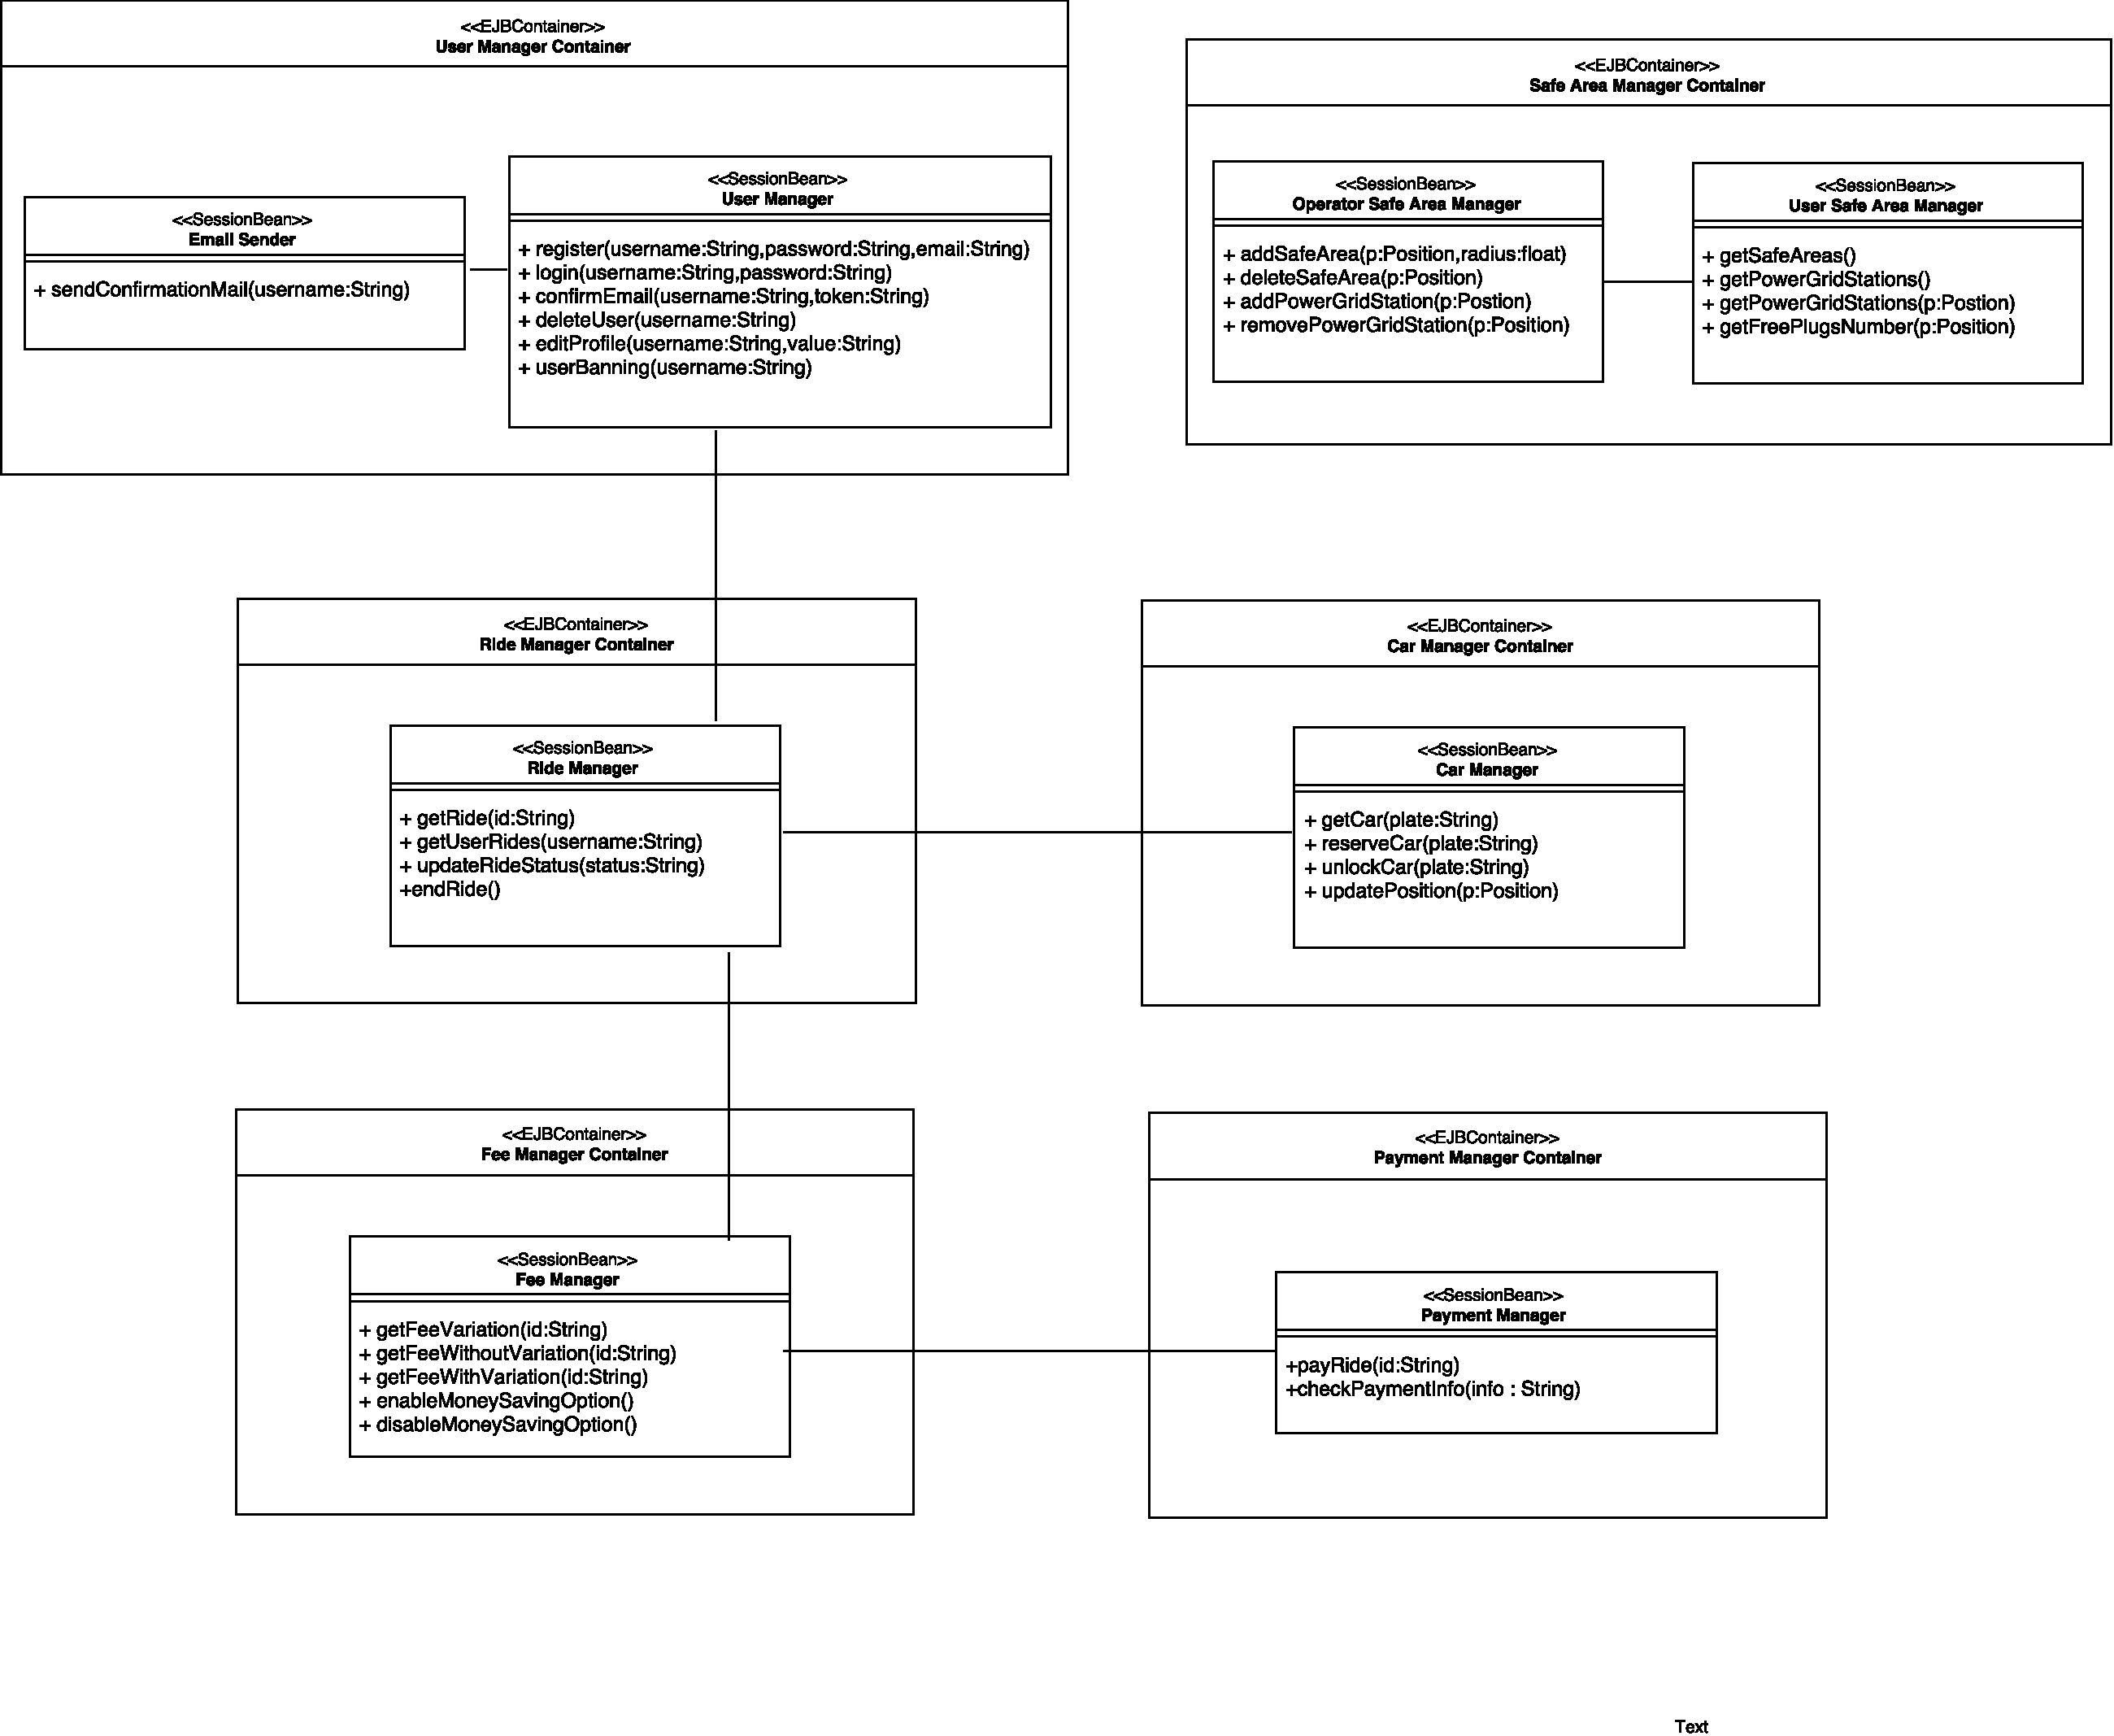
\includepdf{architectural_design/Architecture_Diagrams/SessionBeans.pdf}


